\section{Bản vẽ thiết kế và Mô hình 3D}

Nhằm đảm bảo sản phẩm hoạt động ổn định và mang tính thẩm mỹ cao trên bàn học, nhóm đã tiến hành thiết kế vỏ hộp bảo vệ chuyên dụng trên phần mềm Autodesk Fusion 360 và thực hiện gia công bằng công nghệ in 3D nhựa ABS.

\subsection{Kích thước tổng thể và kết cấu vỏ hộp}

Hộp thiết bị bao gồm hai phần chính: Thân hộp đáy và Nắp đậy phía trên, được liên kết chắc chắn bằng 4 vít cơ khí M3 tại 4 góc.

\begin{itemize}[leftmargin=0.8cm]
    \item \textbf{Kích thước phủ bì thân hộp:} Chiều dài 150 mm $\times$ Chiều rộng 100 mm $\times$ Chiều cao 47 mm.
    \item \textbf{Độ dày thành và đáy:} Độ dày thành 2.5 mm, độ dày đáy 2.5 mm, bo góc ngoài bán kính R6 mm, bo góc trong bán kính R3.5 mm.
    \item \textbf{Nắp hộp:} Kích thước 150 mm $\times$ 100 mm $\times$ 3.0 mm, gia công 4 lỗ bắt vít âm $\varnothing 3.4$ mm tương ứng với các trụ vít $\varnothing 9$ mm ở thân hộp.
    \item \textbf{Chân đế chống trượt:} Bố trí 4 đệm cao su $\varnothing 10$ mm tại 4 góc mặt đáy để tăng độ bám dính khi đặt trên mặt bàn gỗ hoặc kính.
\end{itemize}

\subsection{Hình ảnh mô hình 3D và bố trí ngoại quan}

Mặt ngoài của hộp được bố trí trực quan giúp người học dễ dàng thao tác quẹt thẻ, quan sát màn hình và điều khiển đèn báo.

\begin{figure}[htbp]
\centering
\begin{subfigure}[b]{0.48\textwidth}
    \centering
    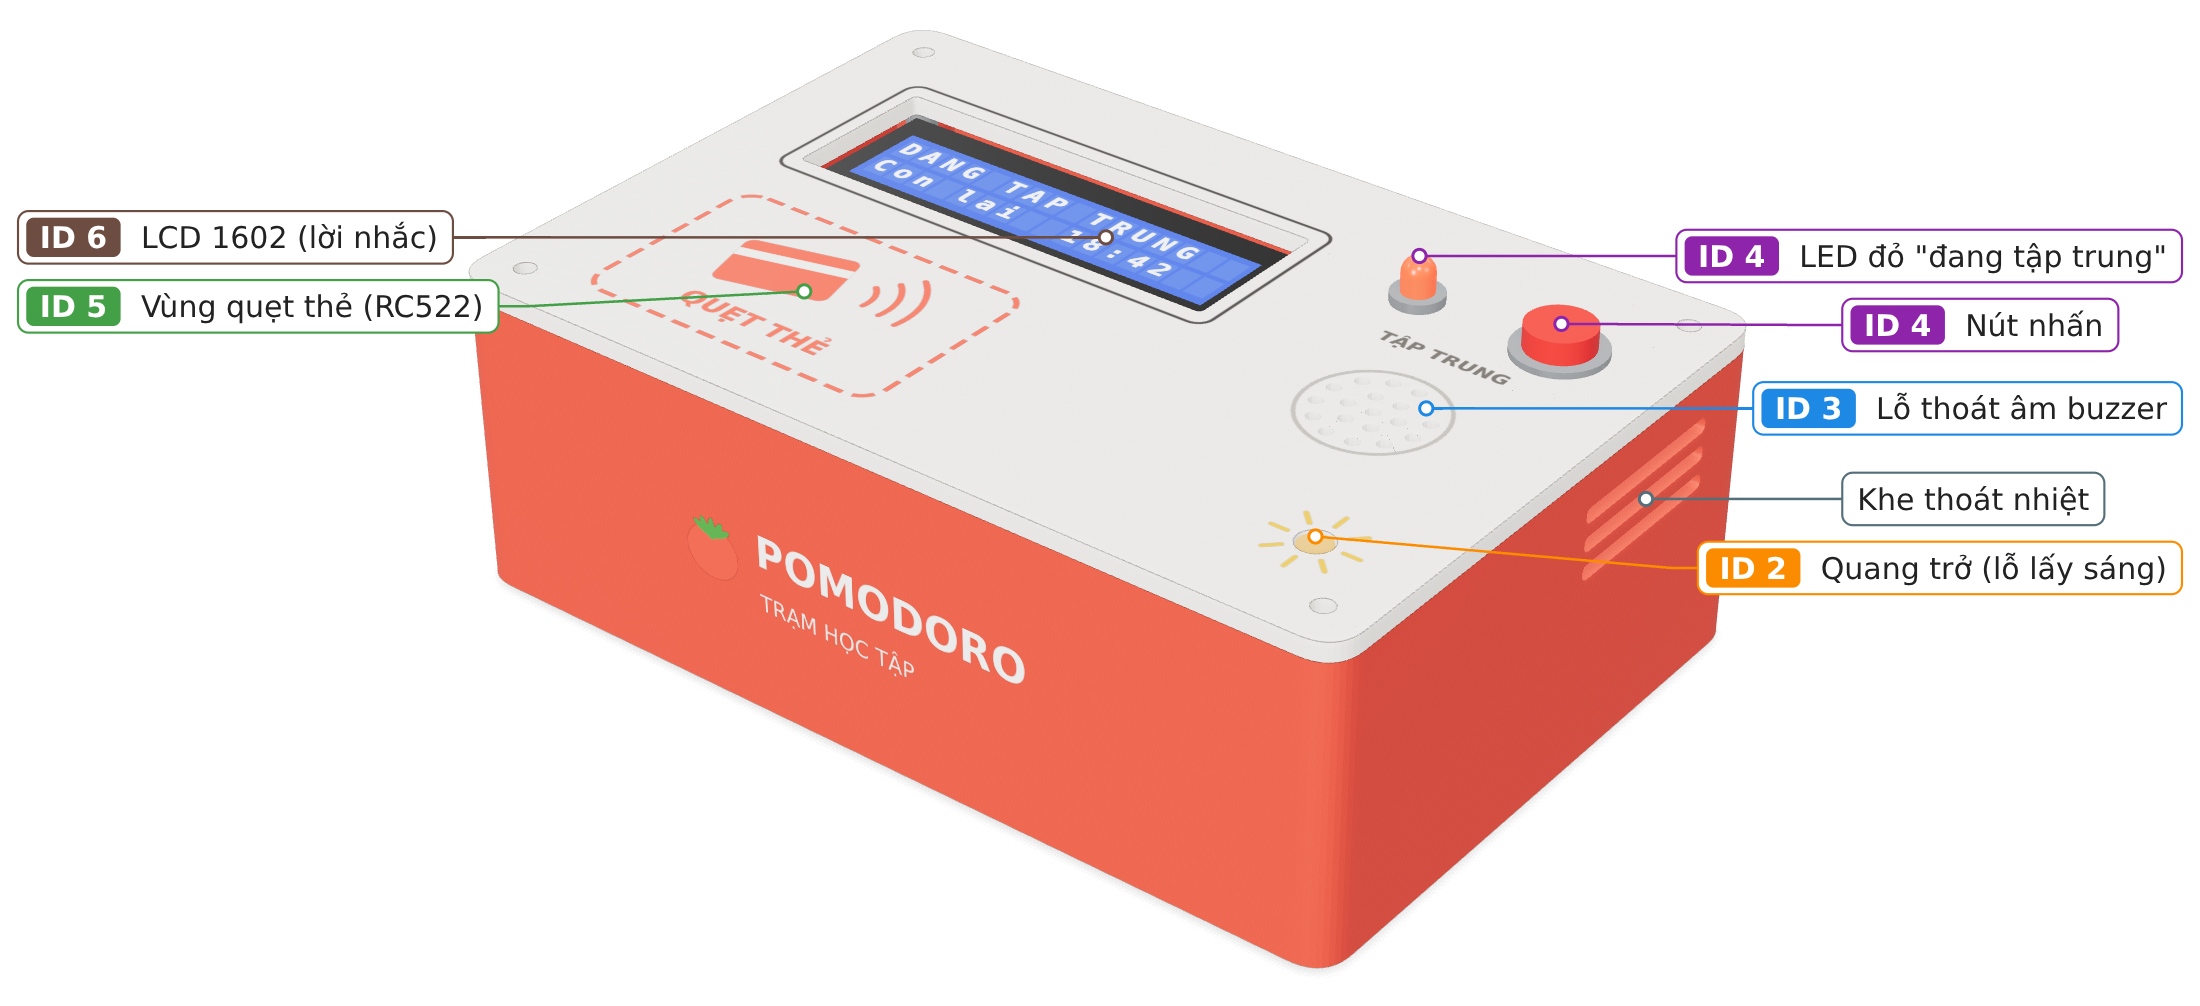
\includegraphics[width=\textwidth]{assets/design/hinh_3d_1_ben_ngoai_truoc.png}
    \caption{Phối cảnh mặt trước trạm học tập}
    \label{fig:3d_front}
\end{subfigure}
\hfill
\begin{subfigure}[b]{0.48\textwidth}
    \centering
    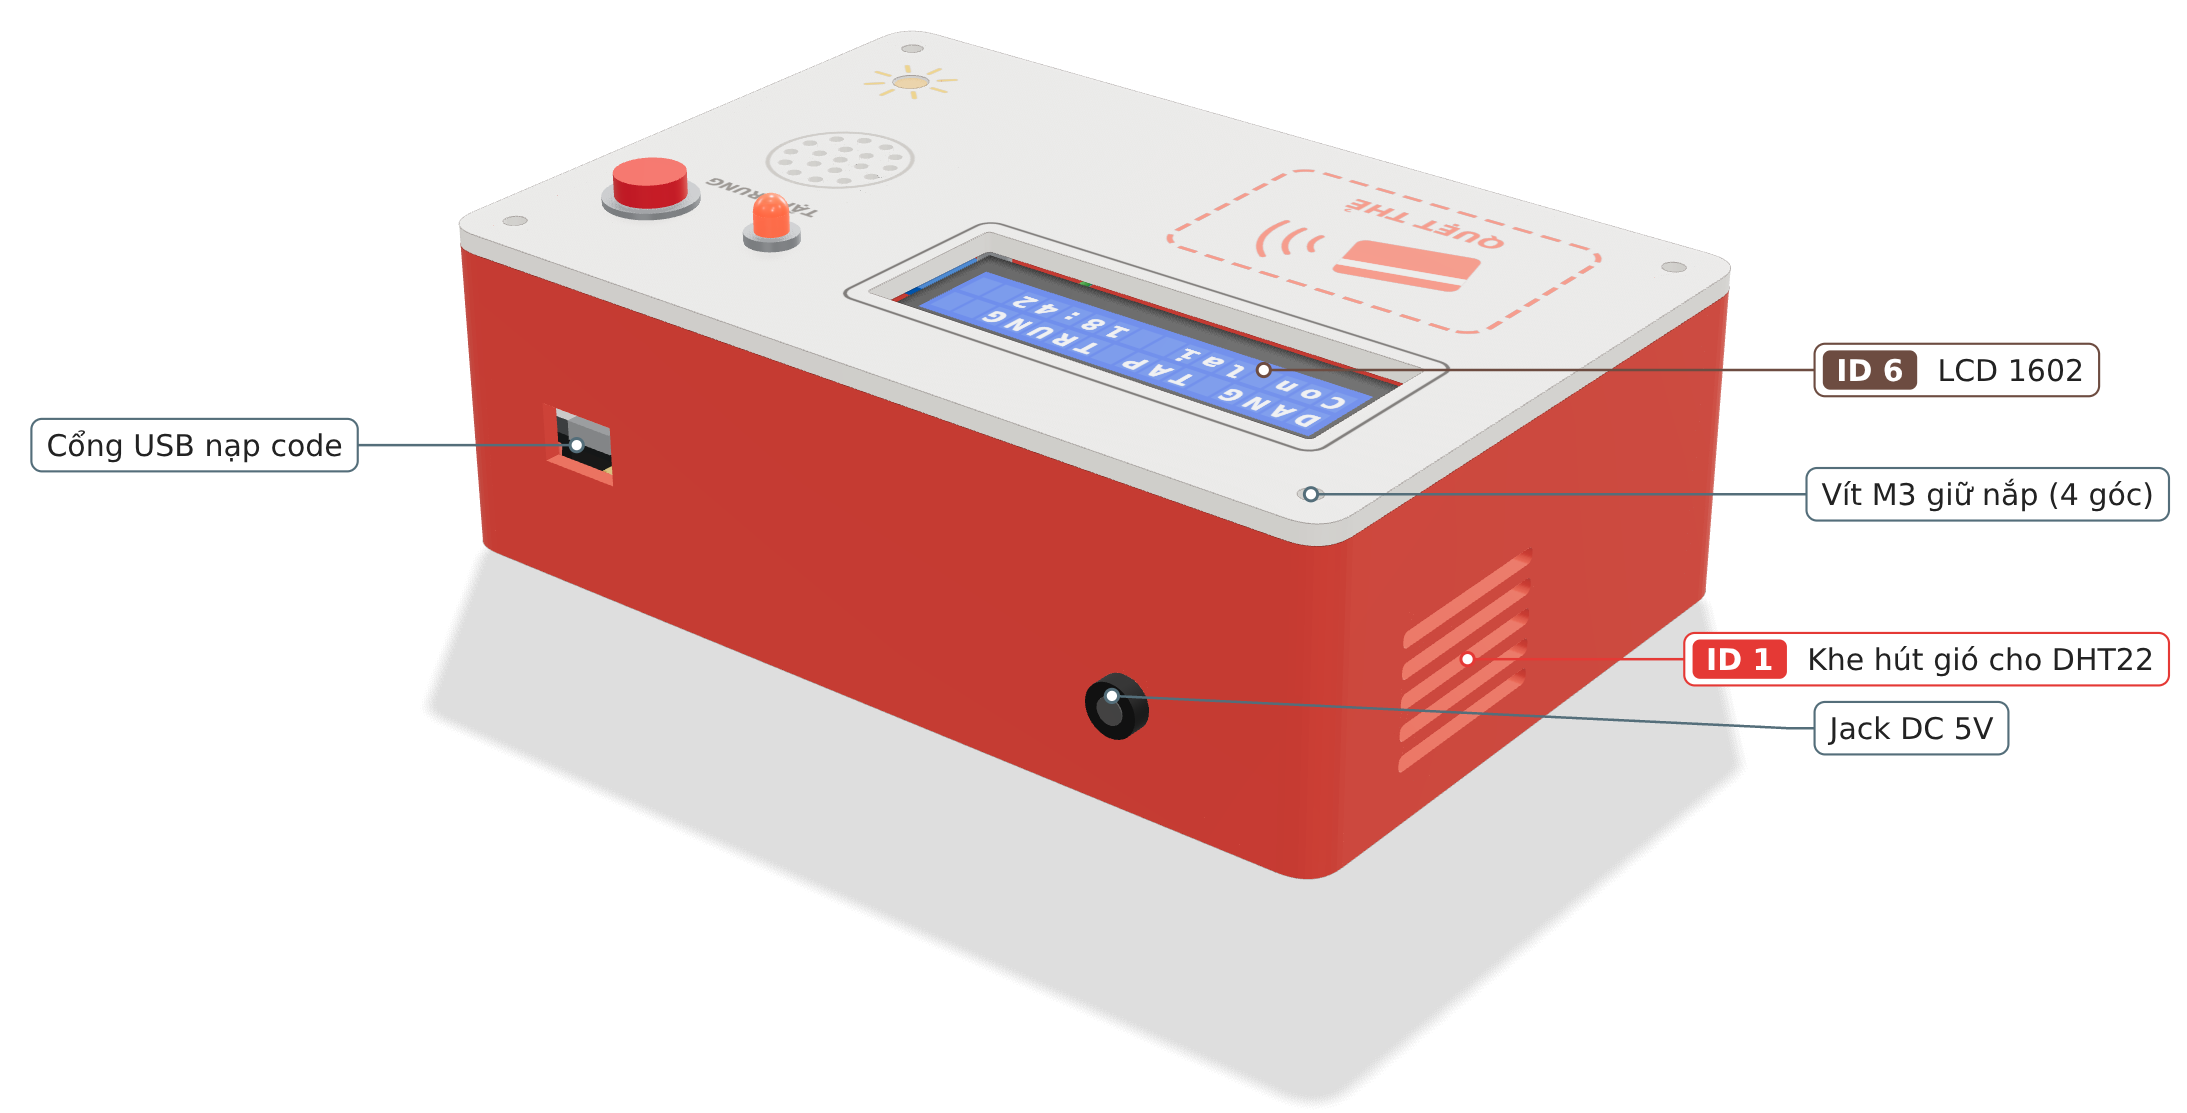
\includegraphics[width=\textwidth]{assets/design/hinh_3d_2_ben_ngoai_sau.png}
    \caption{Phối cảnh mặt sau và các cổng kết nối}
    \label{fig:3d_back}
\end{subfigure}
\caption{Mô hình 3D bên ngoài trạm học tập Pomodoro Box}
\label{fig:3d_exterior}
\end{figure}

\vspace{0.2cm}
\textbf{Bố trí các cổng và lỗ khoét chức năng trên vỏ hộp:}
\begin{itemize}
    \item \textbf{Cửa sổ màn hình LCD 1602:} Kích thước $73 \times 26$ mm tại trung tâm phía trên nắp hộp.
    \item \textbf{Vùng cảm ứng thẻ RFID (RC522):} Kích thước $52 \times 34$ mm tại nửa dưới nắp hộp, được khắc chìm biểu tượng sóng từ trường ``QUẸT THẺ''. Module RC522 dán ngay sát mặt dưới nắp (cách 1 mm) và đọc xuyên qua lớp nhựa 3 mm mà không cần khoét thủng, đảm bảo độ kín và thẩm mỹ.
    \item \textbf{Nút nhấn \& LED đỏ tập trung:} Nút nhấn $\varnothing 12.2$ mm và lỗ giữ chân LED $\varnothing 6.0$ mm đặt ở góc phải phía trên nắp.
    \item \textbf{Lưới thoát âm còi Buzzer:} Cụm 19 lỗ nhỏ $\varnothing 2.2$ mm bố trí hình hoa thị giúp âm thanh còi thoát ra ngoài rõ ràng.
    \item \textbf{Cảm biến ánh sáng:} Lỗ khoét $\varnothing 5.6$ mm đưa đầu quang trở nhô lên bằng phẳng với mặt nắp.
    \item \textbf{Cổng cấp nguồn \& Nạp code:} Mặt sau có lỗ khoét USB $13 \times 9$ mm thẳng hàng với cổng Micro USB của ESP32 để nạp chương trình mà không cần mở hộp, kèm lỗ gắn Jack DC $\varnothing 8$ mm cấp nguồn 5V.
    \item \textbf{Hệ thống tản nhiệt và thông khí đối lưu:} Mặt bên trái có 5 khe hút gió $30 \times 2.4$ mm dành riêng cho cảm biến DHT22; mặt bên phải có 3 khe thoát nhiệt đặt ở vị trí cao để tạo dòng đối lưu không khí tự nhiên.
\end{itemize}

\subsection{Bố trí linh kiện bên trong thân hộp}

Toàn bộ linh kiện bên trong được phân tầng khoa học để tối ưu hóa không gian và ngăn ngừa nhiễu nhiệt:

\begin{figure}[htbp]
\centering
\begin{subfigure}[b]{0.48\textwidth}
    \centering
    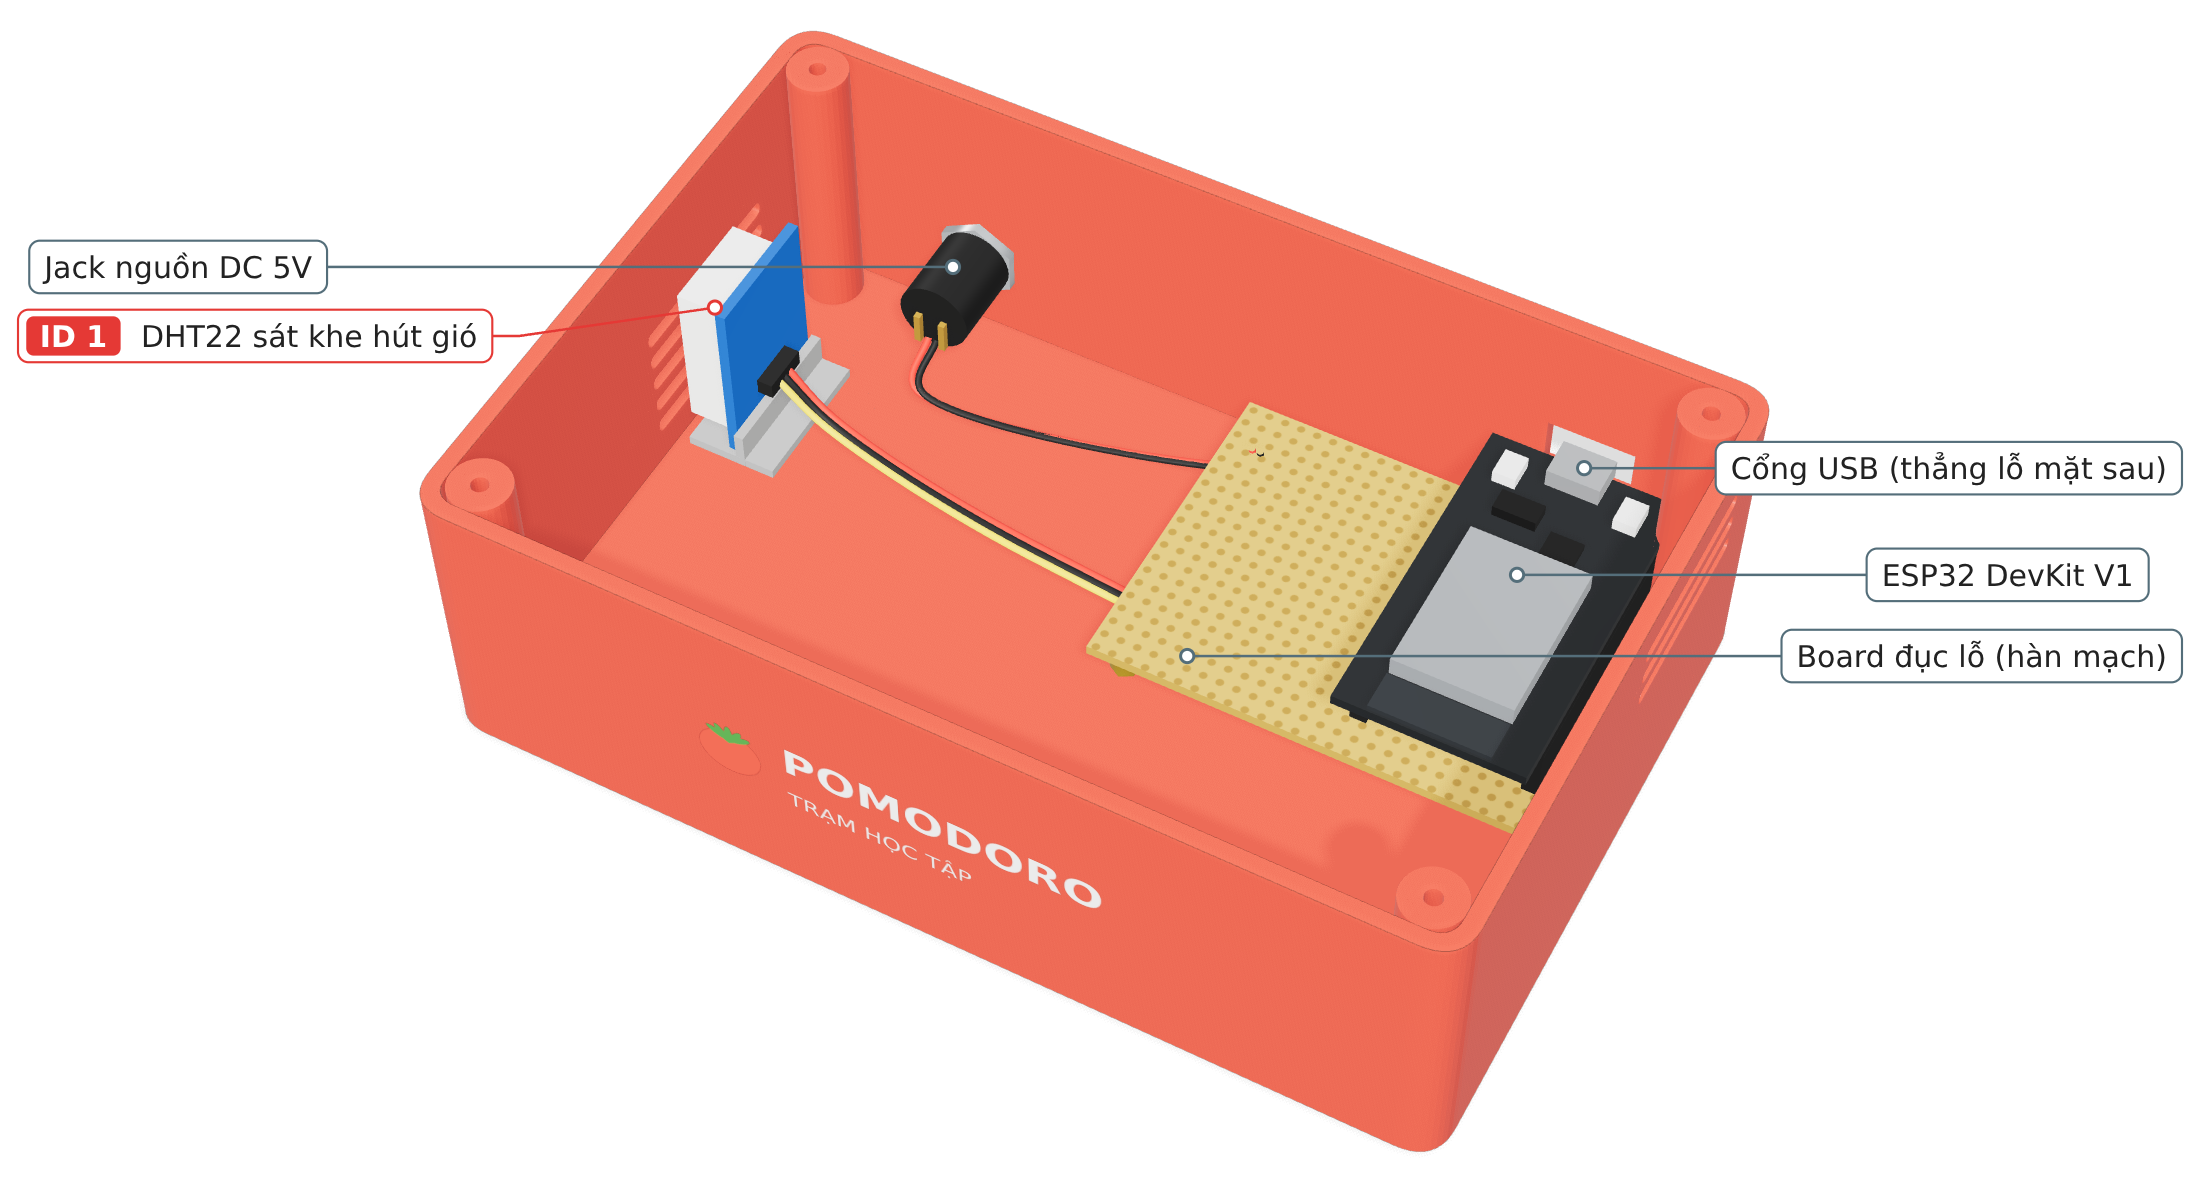
\includegraphics[width=\textwidth]{assets/design/hinh_3d_3_ben_trong_than_hop.png}
    \caption{Bên trong thân hộp đáy}
    \label{fig:3d_inside_body}
\end{subfigure}
\hfill
\begin{subfigure}[b]{0.48\textwidth}
    \centering
    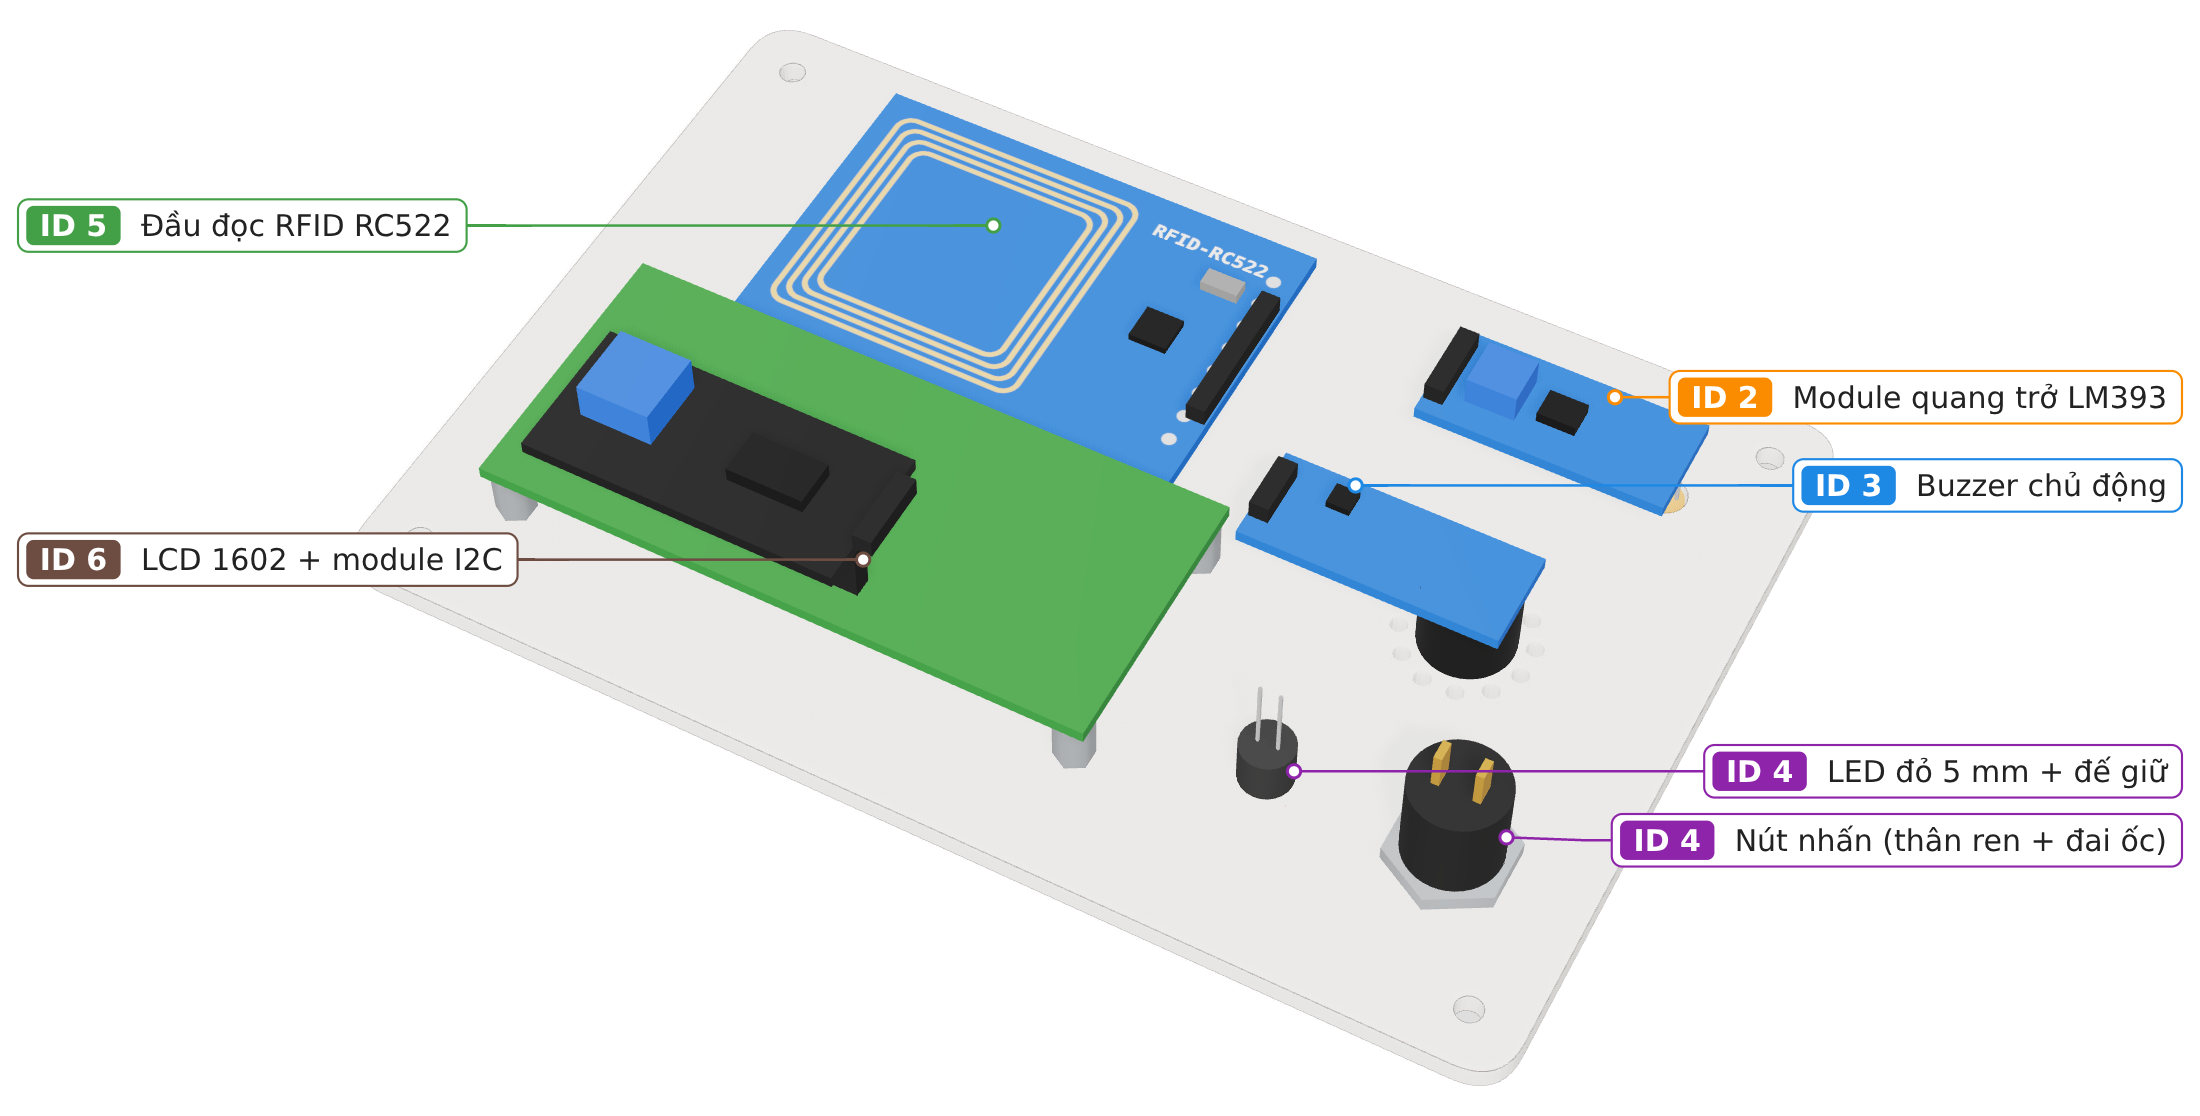
\includegraphics[width=\textwidth]{assets/design/hinh_3d_4_ben_trong_mat_duoi_nap.png}
    \caption{Linh kiện gắn dưới mặt nắp}
    \label{fig:3d_inside_lid}
\end{subfigure}

\vspace{0.4cm}
\begin{subfigure}[b]{0.85\textwidth}
    \centering
    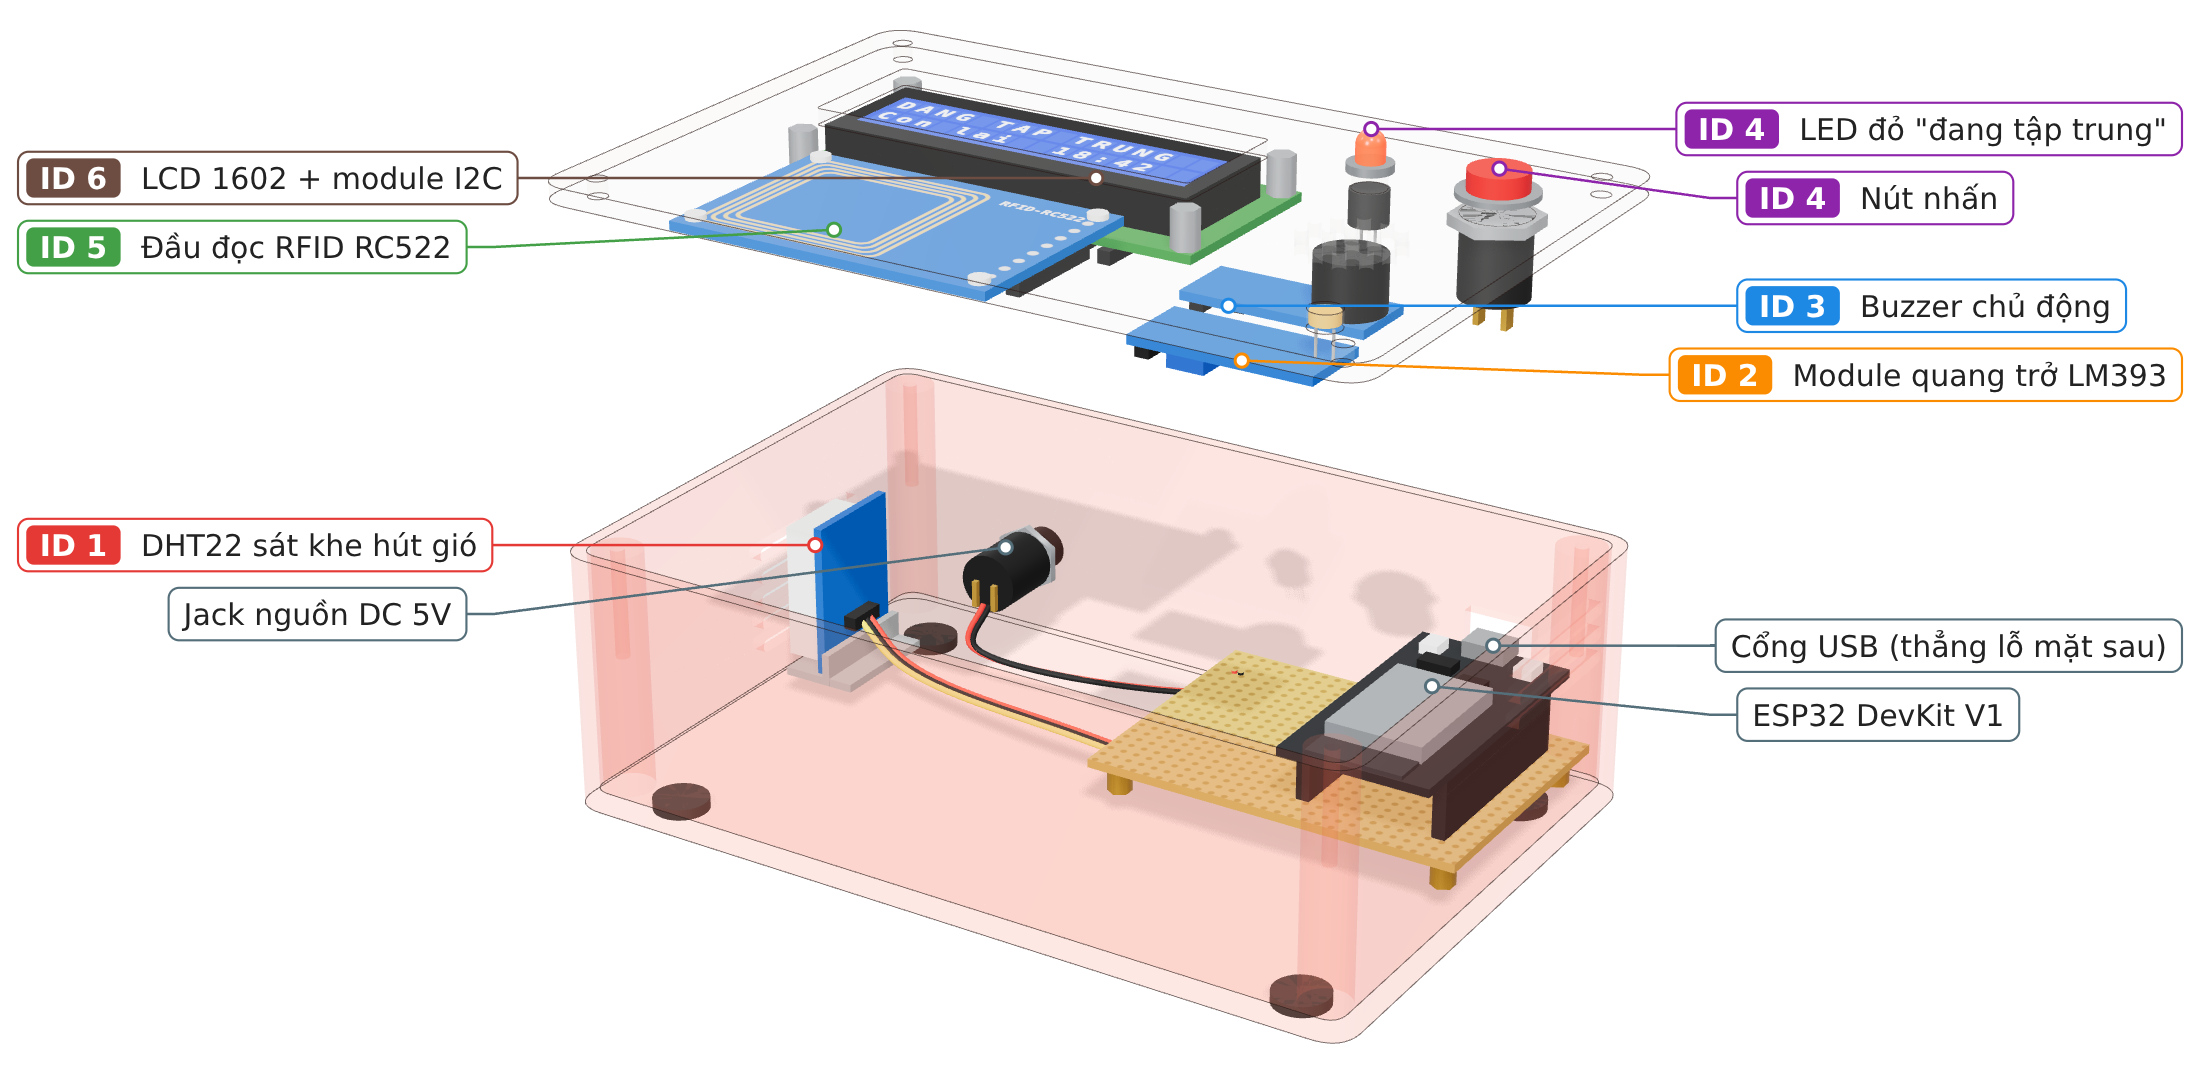
\includegraphics[width=\textwidth]{assets/design/hinh_3d_5_tach_nap.png}
    \caption{Phối cảnh phân rã (Exploded view) toàn bộ kết cấu phần cứng}
    \label{fig:3d_exploded}
\end{subfigure}
\caption{Bố trí phân tầng chi tiết các linh kiện điện tử bên trong trạm học tập}
\label{fig:3d_interior}
\end{figure}

\vspace{0.2cm}
\textbf{Nguyên lý bố trí chống ảnh hưởng lẫn nhau giữa các cảm biến:}
\begin{enumerate}
    \item \textbf{Cách ly nhiệt cho DHT22:} Cảm biến DHT22 được gắn sát thành hộp bên trái, cách xa board vi điều khiển ESP32 khoảng 100 mm. Vị trí này kết hợp với các khe hút gió độc lập giúp số đo nhiệt độ không bị sai lệch bởi nhiệt tỏa ra từ chip ESP32 khi thu phát sóng Wi-Fi.
    \item \textbf{Cách ly quang học:} Module quang trở LM393 đặt cách đèn LED đỏ báo tập trung một khoảng 60 mm để ánh sáng phát ra từ LED không chiếu trực tiếp vào cảm biến gây đo sai cường độ sáng phòng học.
    \item \textbf{Khoảng cách không gian 3 chiều:} Khi đóng nắp hộp, các linh kiện treo ngược dưới nắp (LCD, RC522, nút nhấn) và các linh kiện đặt ở đáy (board mạch đục lỗ, ESP32) có khoảng hở an toàn từ 3 đến 5 mm, tuyệt đối không chạm mạch hoặc gây chập điện.
\end{enumerate}

\subsection{Bản vẽ kích thước chi tiết}

\begin{figure}[htbp]
\centering
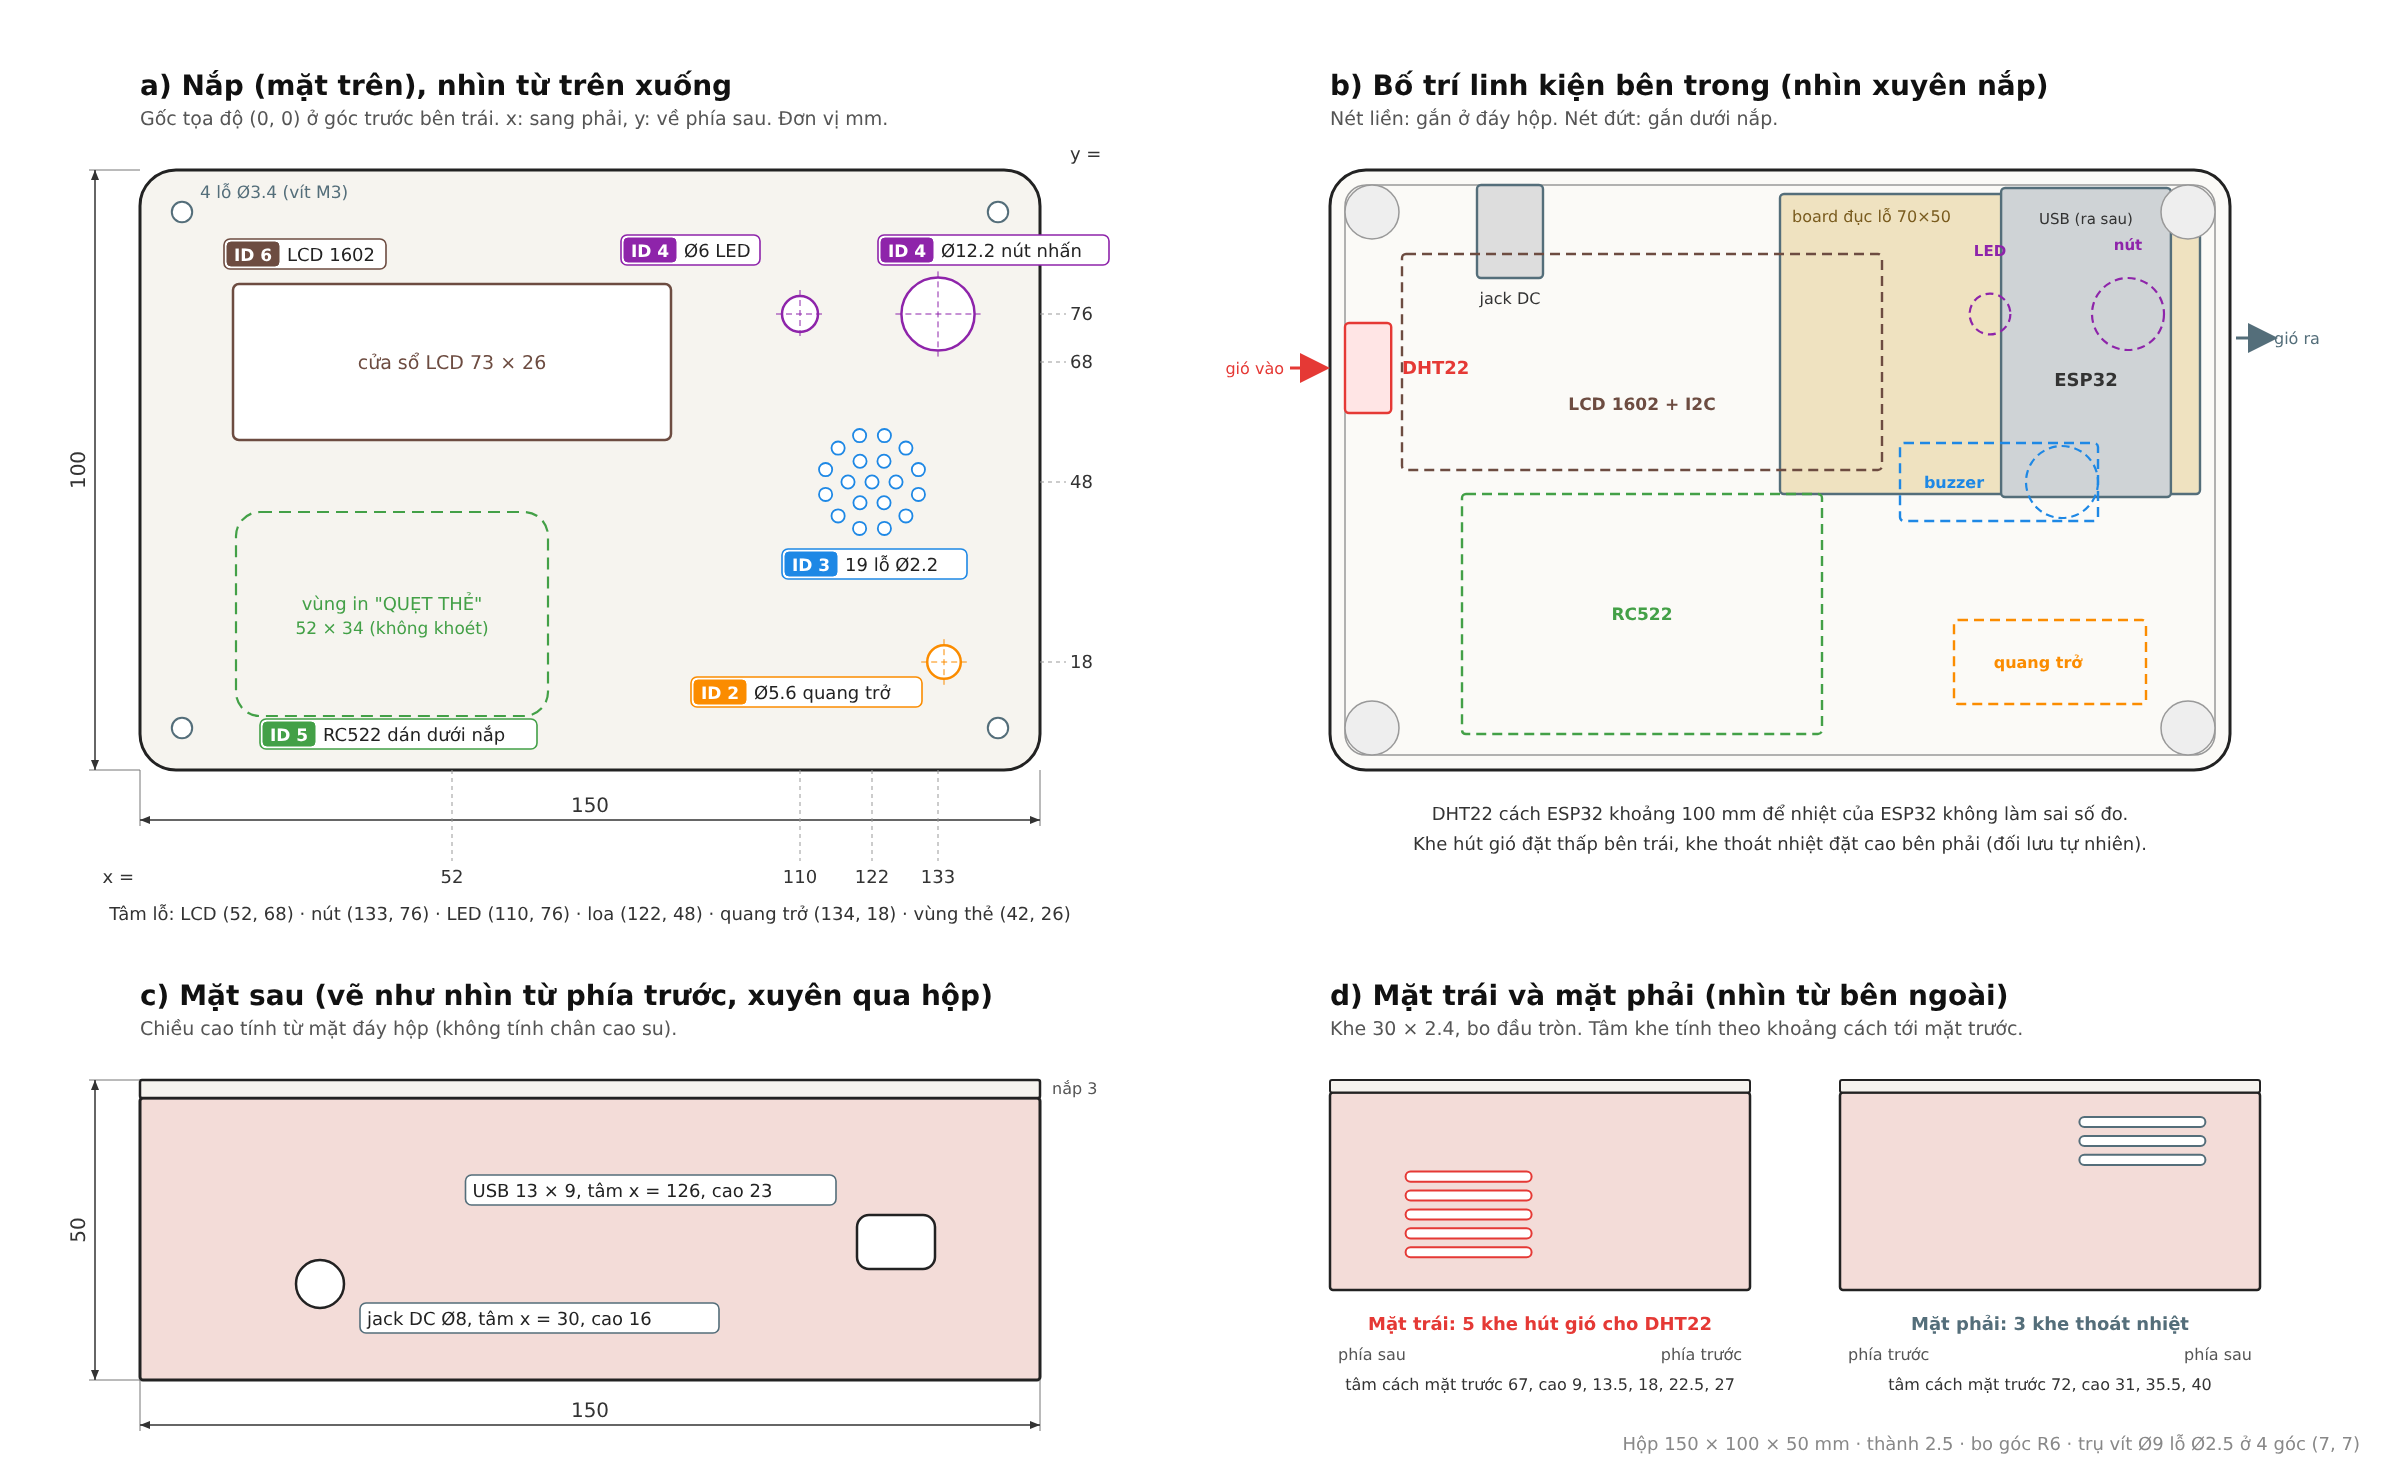
\includegraphics[width=0.95\textwidth]{assets/design/hinh_3d_6_ban_ve_kich_thuoc.png}
\caption{Bản vẽ kỹ thuật 2D kích thước chi tiết các mặt của trạm học tập Pomodoro}
\label{fig:2d_technical_drawing}
\end{figure}
